\section{Calculation of Tsallis Entropy}
\begin{itemize}
\item
Now we calculate the Tsallis generalization of entropy for the state $\rho$ from \eqref{rhomatrix} with a parameter $q \in(0,1) \cup(1, \infty) $. The calculation process is similar to the von Neumann case, up until the function implementation at \eqref{functionimp:1} in which we change the function $F$ to the function  $t$ adapted to \defref{TsallisDEF}:
\begin{align}
\label{functionimp1}
T(q;\rho) &= \frac{1}{1-q} \left\{ \Tr \left[ t(q;\rho) \right] -1   \right\} \\[0.5em]
&= \frac{1}{1-q} \left\{ \Tr \left[ t(q;MDM^{-1}) \right] -1   \right\} \\[0.5em]
&=\frac{1}{1-q} \left\{ \Tr \left[
M
\left( \begin{array}{cccc}
 t(q;1) & 0 & 0 & 0 \\
 0 & t(q;0) & 0 & 0 \\
 0 & 0 & t(q;0) & 0 \\
 0 & 0 & 0 & t(q;0) \\
\end{array}
\right)
M^{-1}
\right]-1
\right\}
\nonumber\\[0.5em]
&=\frac{1}{1-q} \left\{ \Tr \left[
M
\left( \begin{array}{cccc}
 1^{q} & 0 & 0 & 0 \\
 0 & 0^{q} & 0 & 0 \\
 0 & 0 & 0^{q} & 0 \\
 0 & 0 & 0 & 0^{q} \\
\end{array}
\right)
M^{-1}
\right]-1
\right\}
\nonumber\\[0.5em]
&=\frac{1}{1-q} \left\{ \frac{1}{2} \Tr \left[ \left(
\begin{array}{cccc}
 0 & 0 & 0 & 0 \\
 0 & 1 & i & 0 \\
 0 & -i & 1 & 0 \\
 0 & 0 & 0 & 0 \\
\end{array}
\right) \right] -1
\right\} \\[0.5em]
&=0
\end{align}
This is of course expected since the  Tsallis entropy has a minimum value of $0$ iff $\rho$ is a pure state. 
\item
Let's calculate now the Tsallis entropy of the diagonal density matrix $\rho$ in \eqref{ffrefer} using both $0<s<1$ and $q \in(0,1) \cup(1, \infty)$ as free parameters:
\begin{align}
T(q;\rho(s)) 
&= \frac{1}{1-q} \left \{ \Tr \left[ t(q;\rho(s)) \right]-1 \right\} \\[0.5em]
&= \frac{1}{1-q} \left\{  \Tr \left[ \left(
\begin{array}{cc}
 t(q;s) & 0 \\
 0 & t(q;1-s) \\[0.5em]
\end{array}
\right) \right]-1 \right\}\\[0.5em]
&=
\frac{1}{1-q} \left\{  \Tr \left[ \left(
\begin{array}{cc}
 s^{q} & 0 \\
 0 & (1-s)^{q} \\[0.5em]
\end{array}
\right) \right]-1 \right\} \\[0.5em] 
&=\frac{\left[ s^{q }+(1-s)^{q }-1 \right]}{1-q}
\end{align}
Let's plot for different values of q:
\begin{figure}[H]
\begin{center}
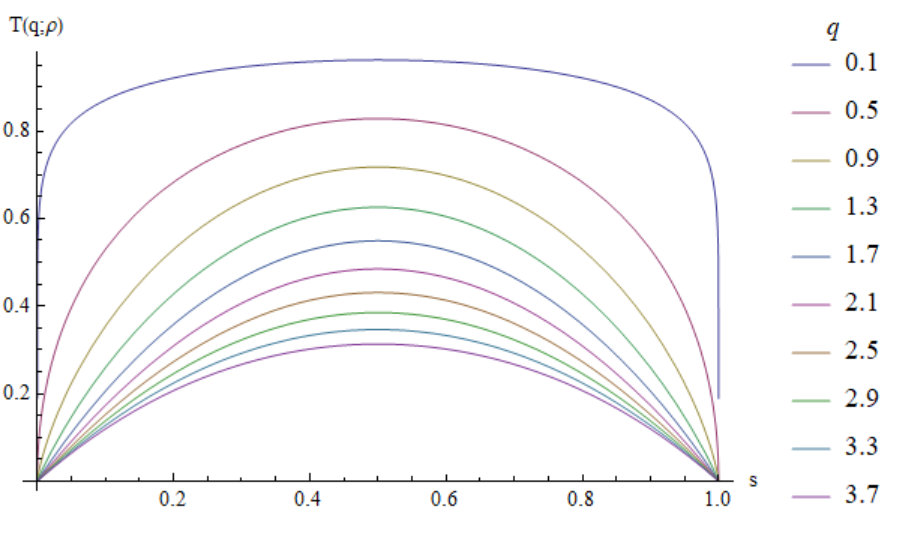
\includegraphics[scale=0.8]{figures/tsallis_ent_plot.png}
\caption{Two points to make: (a)$\lim_{q \to 1}T(q;\rho) = S(\rho)$ is demonstrated via the similarities with figure \ref{figure1}, (b) for $s=0.5$ Tsallis entropy is not independent of q.}
\end{center}
\end{figure}
and in $3D$ for more intuition:
\begin{figure}[H]
\begin{center}
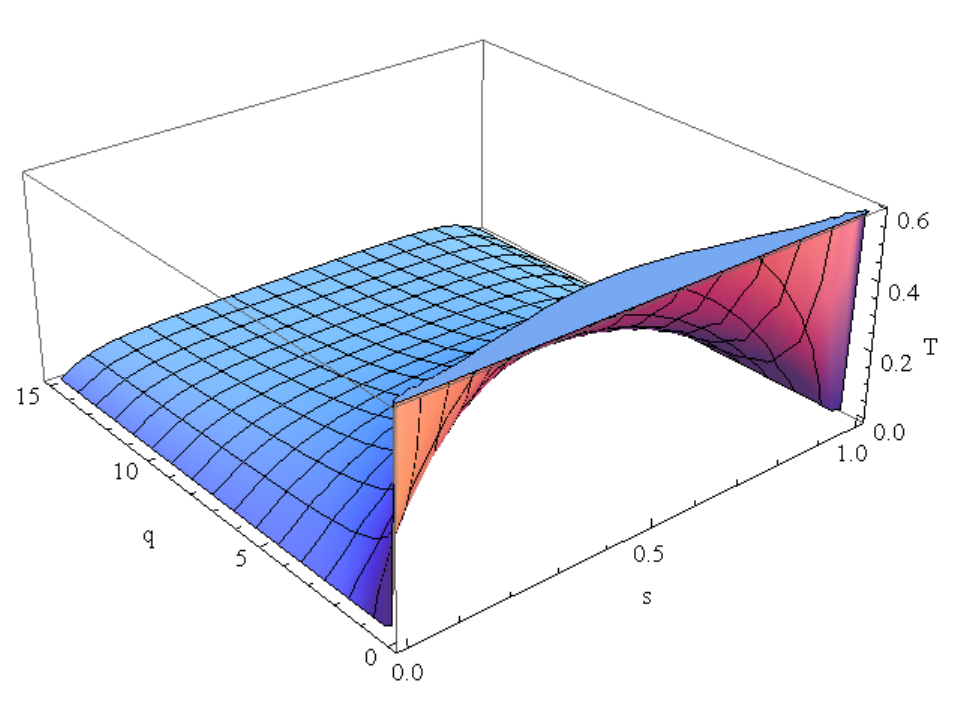
\includegraphics[scale=0.8]{figures/tsallis_ent_plot_3D.png}
\caption{The 3-D plot based on the parameters $s$ and $q$.}\label{figuridiont2}
\end{center}
\end{figure}
Regarding the example \eqref{asdasdas} for maximally mixed eigenvalues $\rho_i=N^{-1}$:
\begin{equation}
T(q;\rho)=\frac{1-N^{1-q}}{q-1}
\end{equation}
\end{itemize}
